\documentclass[manuscript,review,anonymous,nonacm]{acmart}

\AtBeginDocument{%
  \providecommand\BibTeX{{%
    \normalfont B\kern-0.5em{\scshape i\kern-0.25em b}\kern-0.8em\TeX}}}

\setcopyright{none}
\copyrightyear{2026}
\acmYear{2026}
\acmDOI{}

\acmConference[SIGGRAPH Asia '26 Art Papers]{SIGGRAPH Asia 2026 Art Papers}{December 1--4, 2026}{Kuala Lumpur, Malaysia}
\acmBooktitle{SIGGRAPH Asia 2026 Art Papers, December 1--4, 2026, Kuala Lumpur, Malaysia}

\usepackage{multirow}

\begin{document}

\title{Naming the Inexplicable: An Apparatus for Carrying a Y\=okai Until It Fades}

\author{Anonymous for Review}
\email{anon@example.com}
\affiliation{%
  \institution{Anonymous}
  \city{City}
  \country{Country}
}

\renewcommand{\shortauthors}{Anonymous}


%%% ━━━━━━━━━━━━━━━━━━━━━━━━━━━━━━━━━━━
%%% ABSTRACT
%%% ━━━━━━━━━━━━━━━━━━━━━━━━━━━━━━━━━━━
\begin{abstract}
\textit{Y\=okai} is a centuries-old Japanese category through which strange or unexplained experiences are placed in a shared cultural vocabulary. An experience is given a name, a typical place and time, and a short account. Travelers, villagers, regional ethnographers, woodblock artists, and folklorists have each contributed entries to this category over time. The setting in which an ordinary person contributes a new entry, however, has nearly left contemporary life: \textit{y\=okai} are encountered today as finished entries in museums and commercial works, and the publicly available \textit{y\=okai} digital archive is consulted for reference rather than used as a substrate for new cultural production.

This paper asks what enters the \textit{y\=okai} category when a contemporary individual is given technical means to extend it. We describe an apparatus that performs the \textit{y\=okai}-naming act in three to five minutes. The participant fills a short conversational form whose questions are designed around recurring features in the historical entries (when, where, what was sensed, what disposition it leaves); the apparatus retrieves related historical entries from the digital archive, then proposes candidate names, narratives, and images in folkloric register, which the participant accepts, modifies, or rejects.

Across this deployment, the apparatus produced 66 entries. We report what was produced, what participants said about the experience, and what a small group of entries with no clear precedent in the corpus suggests about where contemporary unease accumulates. We discuss the corpus-bias and population-bias caveats that constrain interpretation.
\end{abstract}

\begin{CCSXML}
<ccs2012>
   <concept>
       <concept_id>10010405.10010469.10010474</concept_id>
       <concept_desc>Applied computing~Media arts</concept_desc>
       <concept_significance>700</concept_significance>
   </concept>
   <concept>
       <concept_id>10010405.10010469.10010475</concept_id>
       <concept_desc>Applied computing~Digital libraries and archives</concept_desc>
       <concept_significance>300</concept_significance>
   </concept>
   <concept>
       <concept_id>10003120.10003121.10003124.10010870</concept_id>
       <concept_desc>Human-centered computing~Interaction design</concept_desc>
       <concept_significance>200</concept_significance>
   </concept>
</ccs2012>
\end{CCSXML}

\ccsdesc[700]{Applied computing~Media arts}
\ccsdesc[300]{Applied computing~Digital libraries and archives}
\ccsdesc[200]{Human-centered computing~Interaction design}

\keywords{Computational Folkloristics, Generative AI, Intangible Cultural Heritage, Y\=okai, Ephemeral Materialization, Practice-Based Research}

\begin{teaserfigure}
  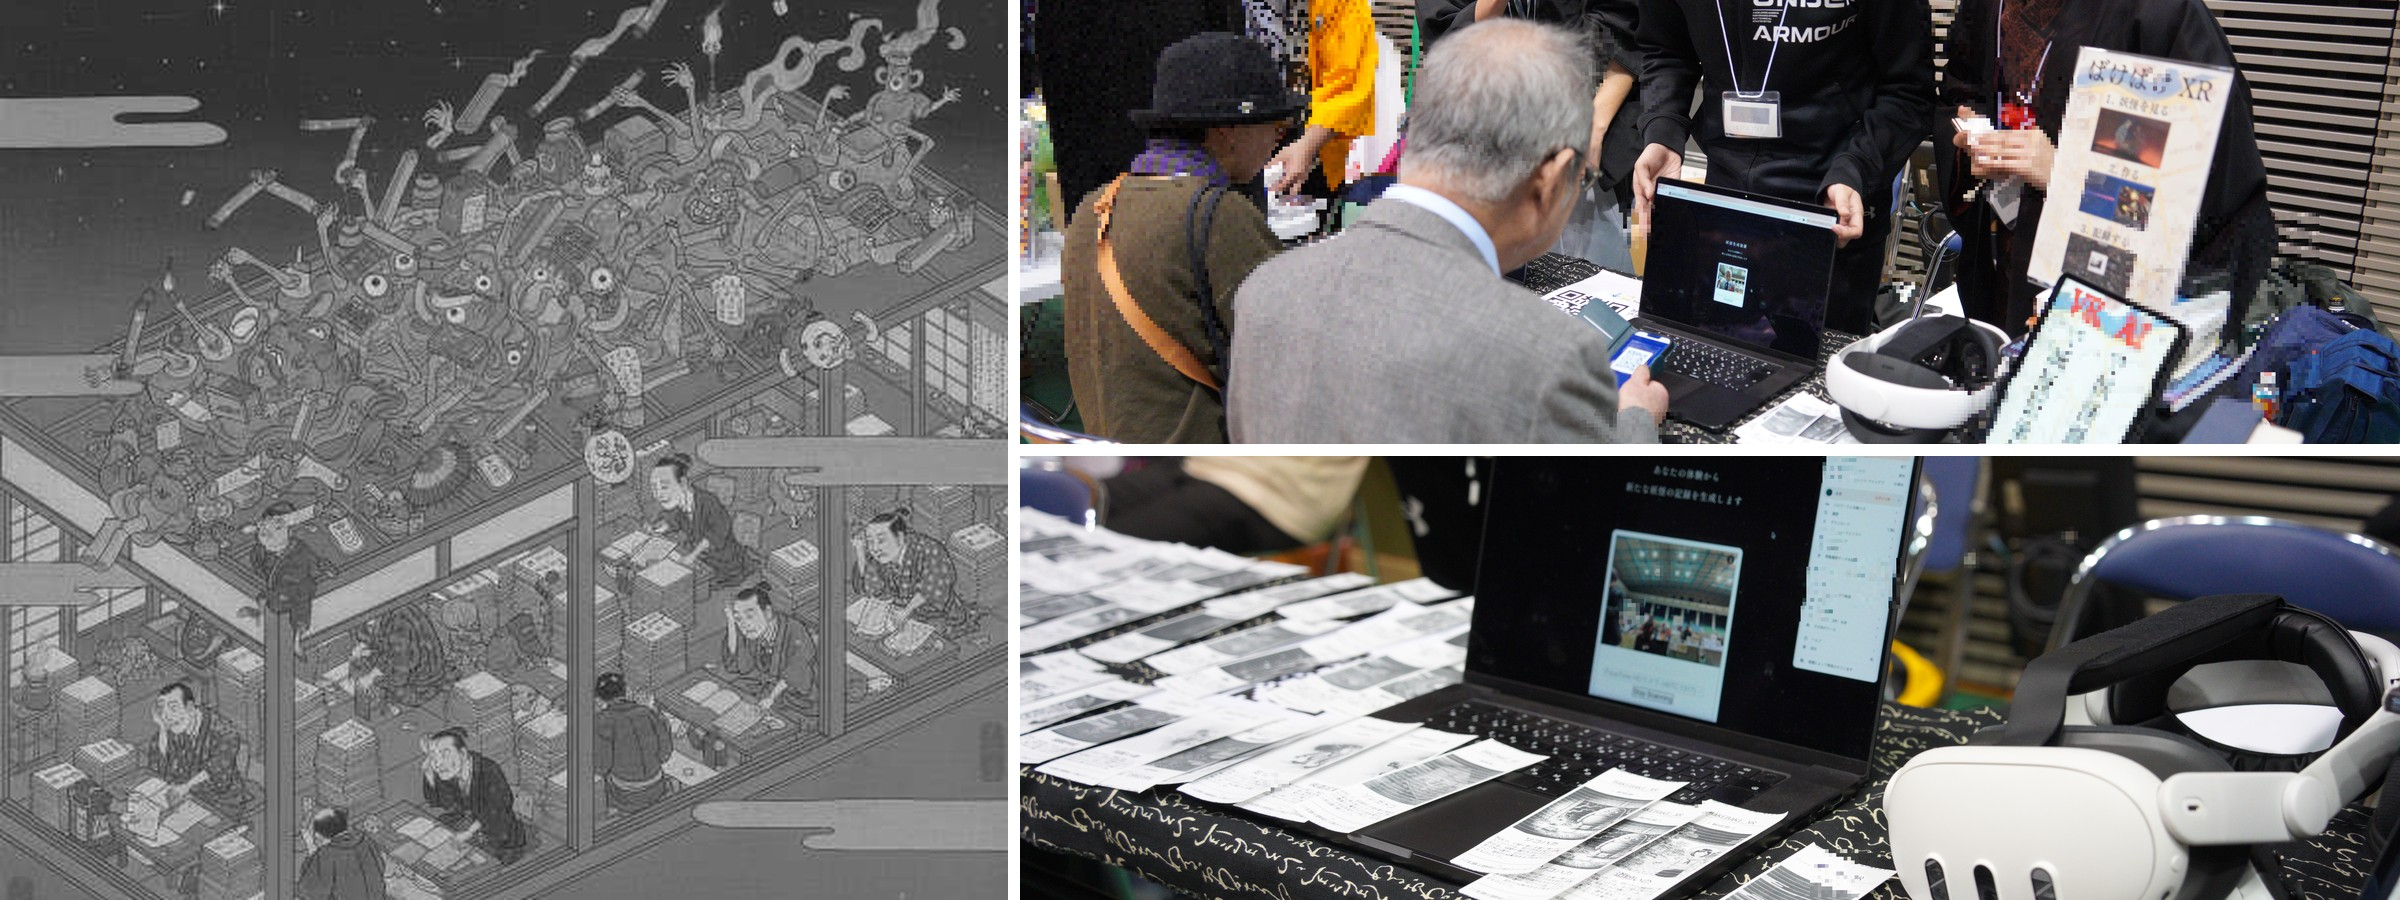
\includegraphics[width=\textwidth]{figures/fig1_teaser.jpg}
  \caption{\textbf{Left}: \textit{Z\=oshoku-zangy\=o} (Multiplying Overtime), one of the five generated \textit{y\=okai} reported in Section~4.2 whose phenomenon has no precedent in the 35{,}305-entry historical corpus; the depiction places the named experience in the inherited woodblock register. \textbf{Right}: the apparatus in operation at YOKAI EXPO 2026 on Shodoshima Island. Participants describe their own unexplained experience to the apparatus, which proposes a name and a depiction and prints the entry on thermal paper; the receipts (lower right) fade over months. Participant faces are blurred for anonymity.}
  \label{fig:teaser}
\end{teaserfigure}

\maketitle


%%% ━━━━━━━━━━━━━━━━━━━━━━━━━━━━━━━━━━━
%%% 1. INTRODUCTION
%%% ━━━━━━━━━━━━━━━━━━━━━━━━━━━━━━━━━━━
\section{Introduction}

Japanese \textit{y\=okai} is the folkloric tradition that gives a name and a form to unexplained experience. Some of its elements resemble Western ghost lore and other supernatural folklore. For example, a traveler walking on a dark night road hears soft footsteps keeping pace behind them, but no one is there when they look back. The tradition names this presence \textit{Betobetosan}, after the onomatopoeic sound of soft footsteps~\cite{yanagita1956}.

The category has accumulated across periods, from Nara-period (710--794) chronicles~\cite{komatsu2011} and Edo woodblock catalogs~\cite{sekien1776} through Meiji \textit{y\=okai-gaku}~\cite{inoue1893} to postwar manga and contemporary online media~\cite{foster2009,yokai_com}. The Nichibunken (International Research Center for Japanese Studies) \textit{Y\=okai} Database archives 35{,}305 entries from this tradition~\cite{nichibunken_db}. Komatsu reads \textit{y\=okai} as a cultural device for converting inexplicable experience into named cultural objects~\cite{komatsu2017}.

The category persists as content. Miyata showed that \textit{y\=okai}, once thought of as pre-modern and tied to village communities, live on through mass media and urban legends, transformed under the conditions of modern city life~\cite{miyata1985}. What has thinned is the act — an ordinary person articulating their own unexplained experience, naming it, and contributing the entry to the shared vocabulary. Foster identifies that act of naming as central to the taxonomy's continued growth~\cite{foster2015}. The wide availability of digitized \textit{y\=okai} corpora has not restored it; the archive is engaged as a reference resource, not as a substrate for participatory production. Some cognate activity continues at the boundary with \textit{kaidan} cultures and regional revival projects~\cite{ichikawa2014}, but these are exceptions.

This paper asks what enters the category when a contemporary individual is given technical means to extend it (Fig.~\ref{fig:teaser}). We describe an apparatus that performs the \textit{y\=okai}-naming act in three to five minutes and prints the entry on thermal paper that fades over months. Across 79 sessions between February and May 2026, the apparatus produced 66 entries. The system is detailed in Section~3 and the records in Section~4.

%%% ━━━━━━━━━━━━━━━━━━━━━━━━━━━━━━━━━━━
%%% 2. RELATED WORK
%%% ━━━━━━━━━━━━━━━━━━━━━━━━━━━━━━━━━━━
\section{Related Work}

\subsection{Yokai studies: methodology, productive operations, and contemporary continuation}

Yokai studies has developed along two lines. Yanagita's existential folkloristics reads \textit{y\=okai} as relegated gods of past belief~\cite{yanagita1956}; Komatsu's structural anthropology, which Hirota describes as a methodological replacement~\cite{hirota2017}, reads \textit{y\=okai} as a cultural device that converts inexplicable experience into named cultural objects, defined relationally to \textit{kami}~\cite{komatsu2017}. We follow Komatsu: what is scaffolded is the conversion operation, not the recovery of a historical category. Kagawa locates the productive engine of this operation in two moves — the act of naming, which expanded the Edo taxonomy through the seventeenth-century haikai poet network where \textit{y\=okai} names circulated as \textit{haigon} (haiku words)~\cite{kagawa2020,kagawa2022}, and pictorialization, since a \textit{y\=okai} requires a visual form to enter circulation as an object of cultural play~\cite{kagawa2022}. The apparatus implements both.

Contemporary scholarship documents the category's continued life in institutional rather than village settings (schoolchildren's oral folklore~\cite{tsunemitsu1993}; urban-legend and \textit{kaidan} culture~\cite{iikura2025}) and in regional-revival projects that frame \textit{y\=okai}-making as a way of visualizing regional memory~\cite{ichikawa2014}. The contemporary-setting cluster reported in Section~4.2 is read against this established line, not as a system artifact.

\subsection{Computational engagement with the Nichibunken corpus}

The Nichibunken Y\=okai Database~\cite{nichibunken_db} has been engaged computationally in two prior orientations. Sato and Nakawake apply quantitative methods to the same 35{,}305-entry corpus to characterize regional distribution and cluster canonical \textit{y\=okai} types~\cite{sato2020}. Jinnai et al.'s \textit{YokaiEval} uses \textit{y\=okai} from Japanese folktales as ground-truth content for evaluating language-model knowledge~\cite{jinnai2025}. Both orientations are retrospective — the corpus is the object of analysis. The present apparatus uses the same content prospectively, as substrate against which a participant performs the naming act.

\subsection{Constrained generation and ephemeral material form}

Three design decisions in the apparatus draw on prior work. We adopt the AI-as-suggesting-collaborator configuration that Mirowski et al.\ found most effective in language-model-assisted creative work~\cite{mirowski2023}. We follow Ozawa et al.\ in treating material process as a question for machine-generated images~\cite{ozawa2024}. The use of thermal printers as a medium for self-erasing computation was precedented in the School for Poetic Computation's installation~\cite{sfpc_decay}.

What is not yet documented is a system that scaffolds an individual to perform a specific historical folk practice — adding a new entry to a specific historical taxonomy with its naming, narrative, and pictorial conventions — and that materializes the result on a substrate that fades at the timescale of folk transmission. The combination of practice-grounded, individual-scaffolded, taxonomically-constrained, and materially-impermanent is the design space the present work occupies.


%%% ━━━━━━━━━━━━━━━━━━━━━━━━━━━━━━━━━━━
%%% 3. SYSTEM DESIGN
%%% ━━━━━━━━━━━━━━━━━━━━━━━━━━━━━━━━━━━
\section{System Design}

The apparatus presents the participant with a single continuous flow: an unexplained experience is articulated into language, placed against the historical \textit{y\=okai} corpus, given a name and a depiction, and printed on paper. The participant is the source of the experience and the final selector at every stage; generative AI drafts narrative text and renders the image. Figure~\ref{fig:system} summarizes the five computational stages.

\begin{figure*}[t]
  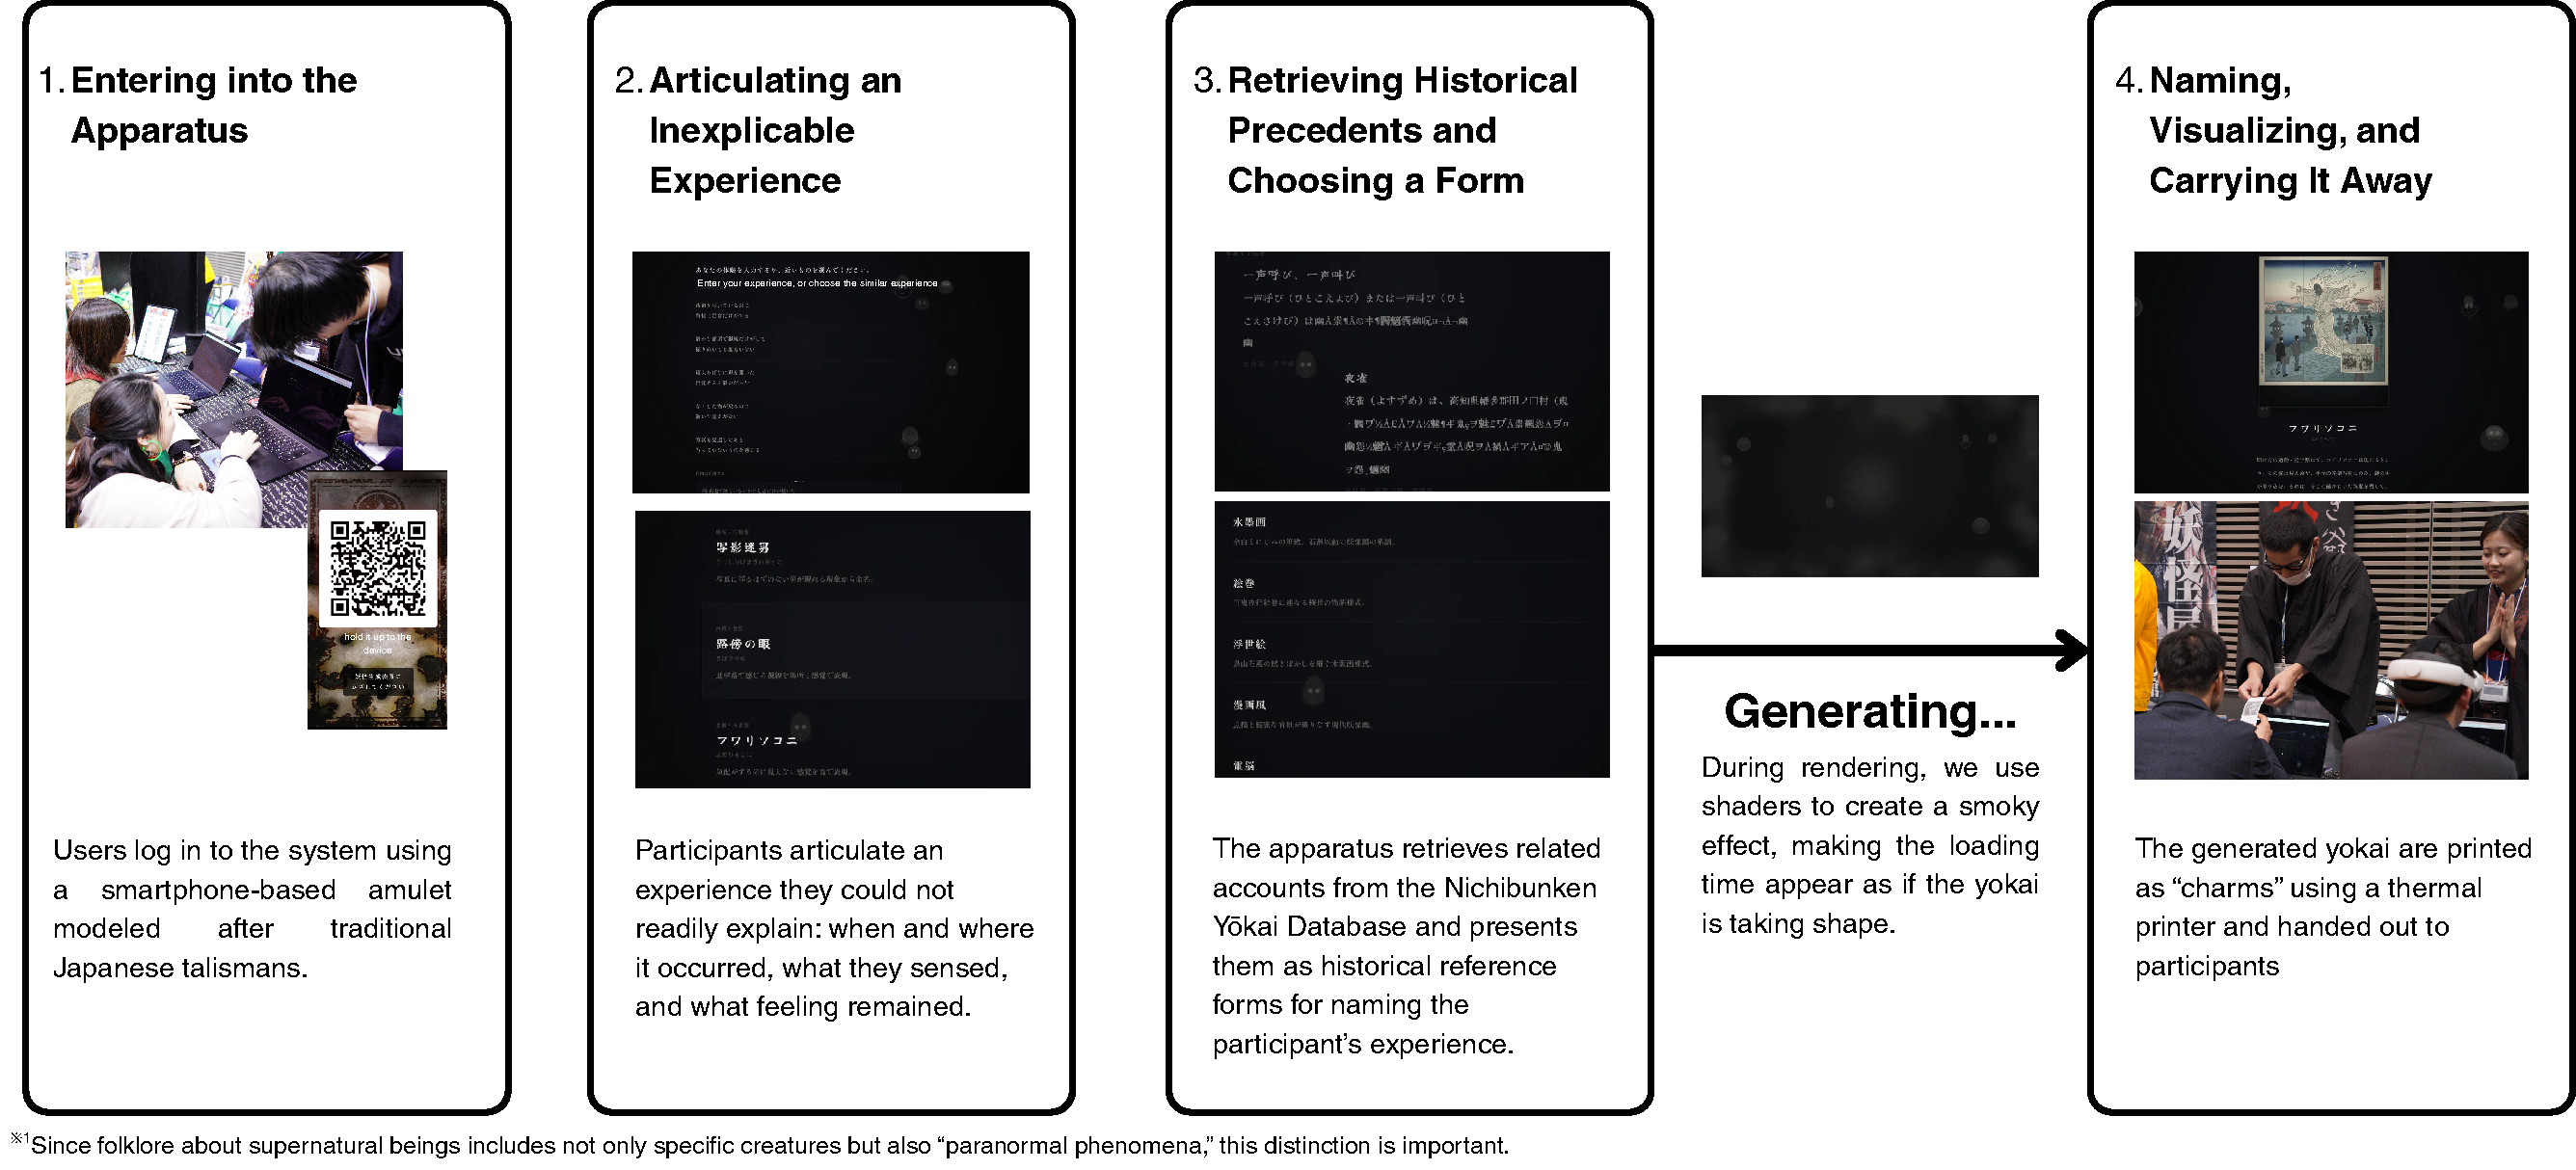
\includegraphics[width=\textwidth]{figures/fig2_system_flow.pdf}
  \caption{The five stages of the apparatus, from open-ended elicitation through retrieval, naming, visualization, and thermal print. The participant articulates the experience and selects from alternatives at each stage; generative AI drafts narrative text and renders the image. Total processing time is three to five minutes per session.}
  \label{fig:system}
\end{figure*}

The participant describes the experience in free text. The form's four prompts (when, where, what was sensed, what disposition was left) were chosen from a corpus-sample coding of where descriptive weight concentrates in historical entries (sentence-position and term-frequency profiles). The participant's own words are carried through every subsequent stage.

The free-text answers are concatenated into a query, embedded via the Gemini Embedding API (768d), and matched by cosine similarity against pre-computed embeddings of the 35{,}305 corpus entries~\cite{nichibunken_db}. The five closest entries are supplied as context to a language model (Gemini 2.0 Flash), which generates three candidate names and short narratives structured along the three naming patterns Komatsu uses to describe the corpus~\cite{komatsu2017} — phenomenon-descriptive, place-conditional, and sensory-onomatopoeic. The model is instructed to reference the retrieved entries without reusing existing names. The participant selects, edits, or supplies a different name.

An image generation model (Google's Nano Banana) then produces a depiction in one of five pictorial registers — ink wash (\textit{suiboku-ga}), illustrated scroll (\textit{emaki}), woodblock print (\textit{ukiyo-e}), narrative ink-line drawing (\textit{manga} and \textit{gekiga}), and contemporary digital. The first four are inherited registers; the fifth is selected for contemporary participant accounts. Each prompt names conventions internal to the chosen register — Sessh\=u's \textit{hatsuboku} line and the eccentric lineage that absorbs \textit{y\=okai} imagery~\cite{tsuji1970}, the procession structure of the \textit{Hyakki Yagy\=o Emaki}~\cite{tanaka1994}, the catalog grammar of Sekien~\cite{sekien1776}, the postwar \textit{gekiga} tradition. Fixing the categorical frame against drift in model defaults follows Walton's argument that an image's representational content depends on the category under which it is perceived~\cite{walton1970}.

\subsection{Materialization}

The output is printed on 80mm thermal receipt paper. The fading substrate is the design line along which the apparatus is built. Thermal ink degrades under ambient light and temperature, and the manufacturer specification indicates legibility on the order of months under typical indoor conditions — approximately the timescale at which a folk telling might be retold a few times before being forgotten. The fade is structural, not a defect: the entry is allowed to disappear as historical entries did before being recorded, and the apparatus does not commit to remembering on the participant's behalf.


%%% ━━━━━━━━━━━━━━━━━━━━━━━━━━━━━━━━━━━
%%% 4. EXHIBITION AND OBSERVATIONS
%%% ━━━━━━━━━━━━━━━━━━━━━━━━━━━━━━━━━━━
\section{Deployment and Records}

\begin{figure}[h]
  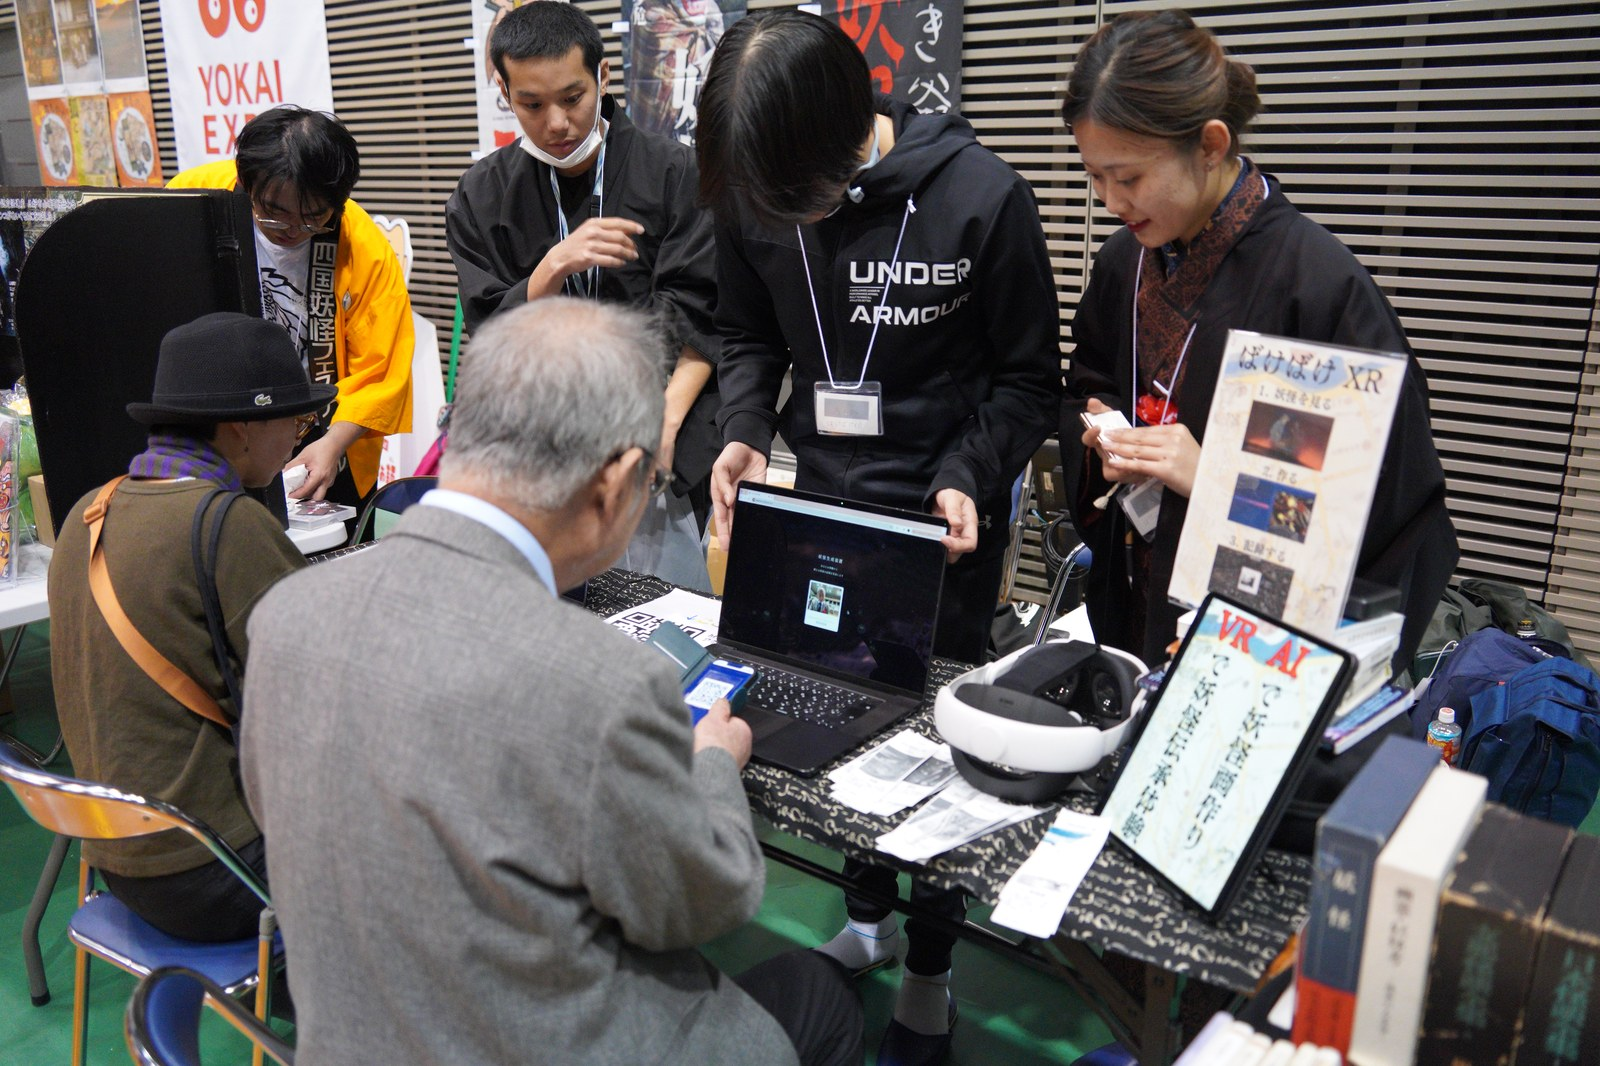
\includegraphics[width=\columnwidth]{figures/fig5_venue.jpg}
  \caption{The apparatus in operation at YOKAI EXPO 2026, Fretopia Hall, Tonosho, Shodoshima Island.}
  \label{fig:venue}
\end{figure}

\subsection{Context and Population}

The apparatus was first deployed at YOKAI EXPO 2026 (Fig.~\ref{fig:venue}), a \textit{y\=okai} festival held on February~22, 2026 at Fretopia Hall on Shodoshima Island, and continued at successive venues through May 2026. Of 79 initiated sessions, 66 produced a complete \textit{y\=okai} (name, narrative, image) and 47 produced a physical receipt. Thirty-seven participants completed both pre- and post-experience surveys. The denominator below is 66 unless otherwise stated; the pre/post category analysis uses the 36 paired surveys with complete responses.

\subsection{What the Apparatus Produced}

\begin{figure*}[t]
  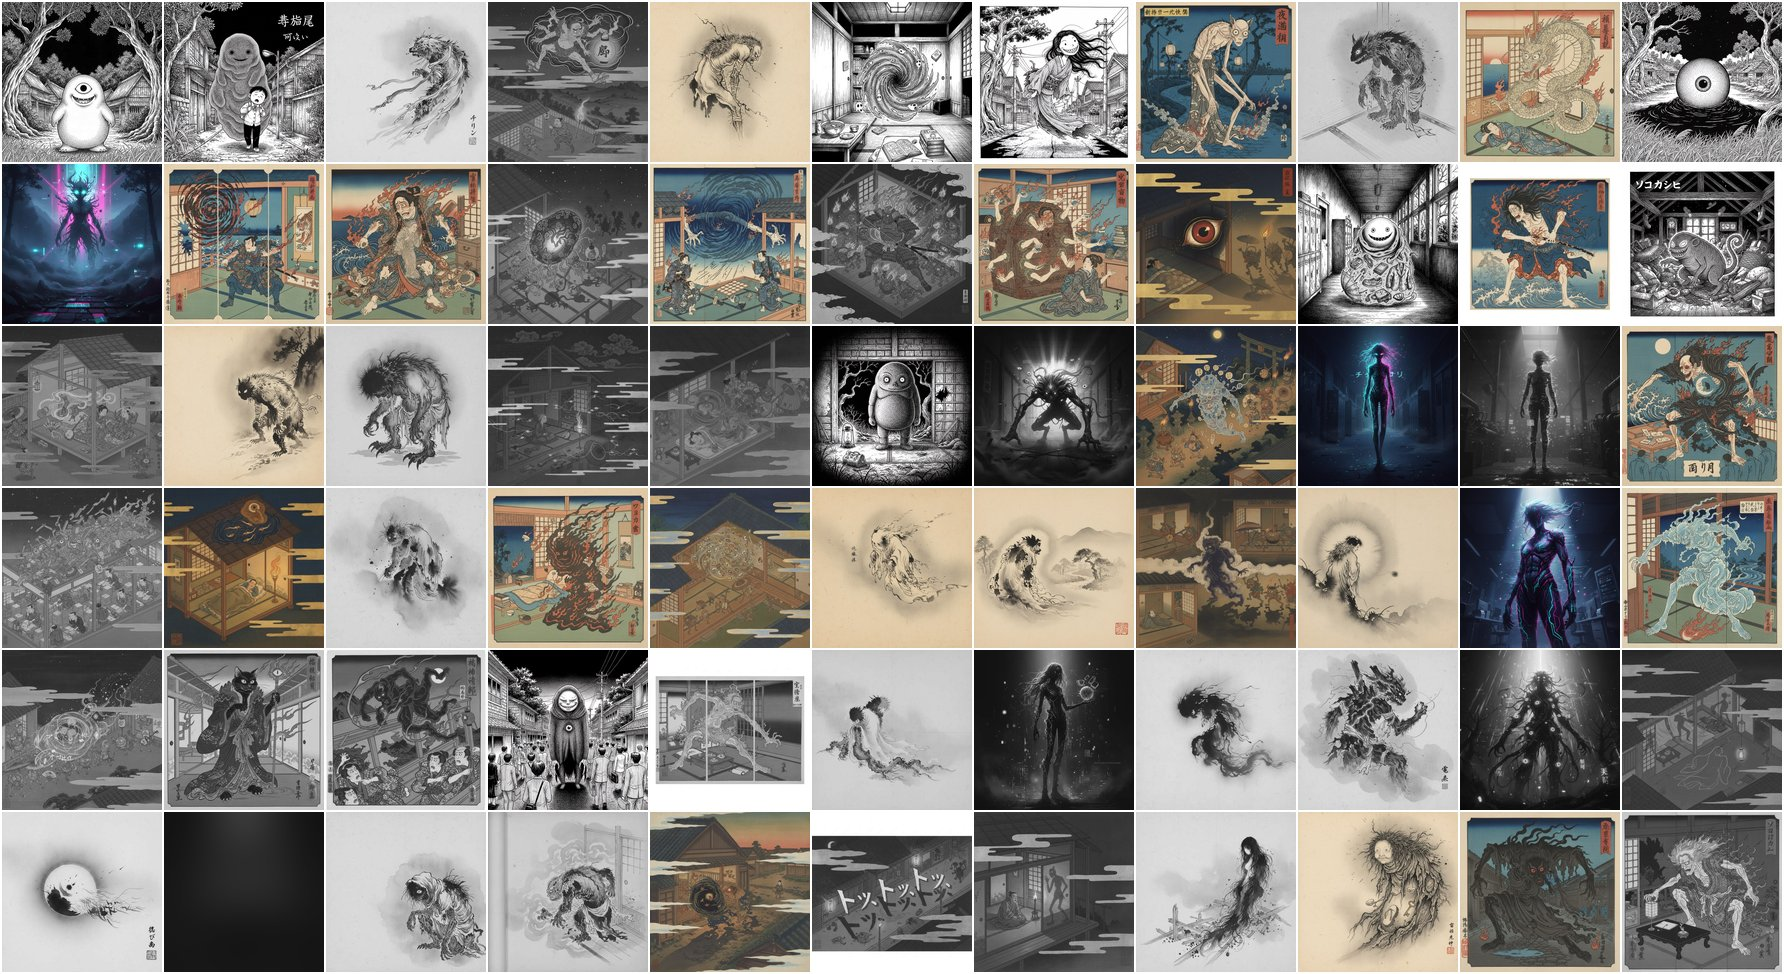
\includegraphics[width=\textwidth]{figures/fig4_atlas.jpg}
  \caption{Atlas of all 66 \textit{y\=okai} produced by the apparatus, in chronological order of generation (left-to-right, top-to-bottom). The inherited pictorial registers (ink wash, woodblock, illustrated scroll) dominate the majority of cells; a sub-cluster of contemporary-digital outputs sits to the right, selected by the apparatus for participant accounts describing contemporary settings. One cell in the bottom-left quadrant is blurred: its output incidentally resembled a well-known copyrighted cartoon character and has been suppressed in the figure while retained in the underlying record.}
  \label{fig:atlas}
\end{figure*}

Figure~\ref{fig:atlas} shows all 66 outputs. Read as a corpus, they cover the structural naming types that organize the historical entries (phenomenon-descriptive, place-conditional, sensory-onomatopoeic) and each entry pairs a place and time with a phenomenon and a named entity in the form the historical corpus has used.

The distribution of settings, however, differed sharply from the historical corpus (Table~\ref{tab:settings}). Settings that have been productive of \textit{y\=okai} across the historical period (home, road, mountain) remained productive in the apparatus output. Settings characteristic of contemporary work and infrastructure (workplace, factory, data audit, electrical infrastructure, event venue, photography) appeared in the apparatus output at rates one to two orders of magnitude above their corpus baseline.

\begin{table}[h]
\caption{Setting vocabulary distribution. Generated \textit{y\=okai} (N=66) versus Nichibunken corpus (N=35{,}305). Categories defined by token lists; one \textit{y\=okai} or entry may match more than one category. Ratio = apparatus rate / corpus rate.}
\label{tab:settings}
\small
\begin{tabular}{lrrr}
\hline
\textbf{Setting} & \textbf{Gen.\%} & \textbf{Corpus \%} & \textbf{Ratio} \\
\hline
home              & 43.9 & 18.13 & 2.4x \\
mountain/wilds    &  9.1 & 22.32 & 0.4x \\
road/path         & 22.7 &  8.89 & 2.6x \\
water             &  1.5 & 17.35 & 0.1x \\
school            & 16.7 &  0.65 & 25.7x \\
workplace/office  &  7.6 &  0.03 & 267.5x \\
factory           &  1.5 &  0.05 & 29.7x \\
photography       &  3.0 &  0.12 & 26.1x \\
event venue       &  1.5 &  0.02 & 66.9x \\
infrastructure    &  1.5 &  0.003 & 534.9x \\
data/audit        &  1.5 &  0.00 & --- \\
\hline
\end{tabular}
\end{table}

The absence of these contemporary settings from the corpus is structural. A token-level search of all 35{,}305 entries returned zero occurrences for the Japanese tokens for overtime, audit, power outage, and photographing.

Eight of the 66 generated \textit{y\=okai} contained setting vocabulary specific to contemporary life (Fig.~\ref{fig:cluster}). Three combined contemporary setting with phenomena that have direct historical analogs (missing objects in the office, peripheral visual presence in photographs, objects returning to their original place at the workplace). The remaining five contain phenomena without precedent in the corpus: \textit{Z\=oshoku-zangy\=o} (Multiplying Overtime) — work multiplies at night as if added by an unseen force; \textit{Kensh\=u-fujun} (Inspection Irregularity) — stagnation enters the audit of records, rates of progress shifting with the auditor's affect; \textit{Dandenh\=ok\=o} (Power-Outage Wandering) — at the moment of an unexpected power loss, a presence draws warmth from those present; \textit{K\=oj\=o-y\=uei} (Factory Dusk-Shadow) — faces are missing from photographs taken at abandoned factories at twilight, with a presence accompanying the absence; \textit{T\=ori-tsuki} (Passing Moon) — the image of a difficult colleague intrudes during work, accompanied by a heaviness that arrests motion. Each was articulated by a visitor as something they had experienced before the encounter; the distinguishing content lies in the phenomenon itself, not in the surface form of the name.

We coded each generated \textit{y\=okai}'s descriptive text along four dimensions (perception, effect, locus, agency) and compared the cluster against the remaining 58 outputs and against a search of the 35{,}305-entry corpus (Table~\ref{tab:codes}). The cluster departs from both the wider output and the corpus on three distinctively contemporary codes: \textbf{drain or erosion} as effect (warmth, attention, or energy taken without identifiable cause); \textbf{multiplication or stagnation} as effect (work that grows, data that does not move); and \textbf{workplace, institutional-data, infrastructure, and photographic loci}, absent from the comparison set.

\begin{table}[h]
\caption{Sensibility coding of generated \textit{y\=okai} descriptions. Percentages are the share of entries in which any token from the code appeared. Corpus column reports the same token search across the 35{,}305-entry Nichibunken corpus.}
\label{tab:codes}
\small
\begin{tabular}{lrrr}
\hline
\textbf{Code} & \textbf{Cluster} & \textbf{Other gen.} & \textbf{Corpus} \\
\hline
perception/invisibility           & 75\% & 59\% & 0.7\% \\
perception/cold                   & 25\% & 16\% & 0.7\% \\
\textbf{effect/drain or erosion}  & \textbf{25\%} & 5\% & 0.5\% \\
\textbf{effect/multiplication}    & \textbf{25\%} & 0\% & 0.3\% \\
\textbf{locus/workplace}          & \textbf{62\%} & 0\% & 0.0\% \\
\textbf{locus/institutional-data} & \textbf{12\%} & 0\% & 0.1\% \\
\textbf{locus/infrastructure}     & \textbf{12\%} & 0\% & 0.0\% \\
\textbf{locus/photographic}       & \textbf{25\%} & 0\% & 0.1\% \\
agency/no-named-cause             & 50\% & 43\% & 1.5\% \\
\hline
\end{tabular}
\end{table}

\begin{figure*}[t]
  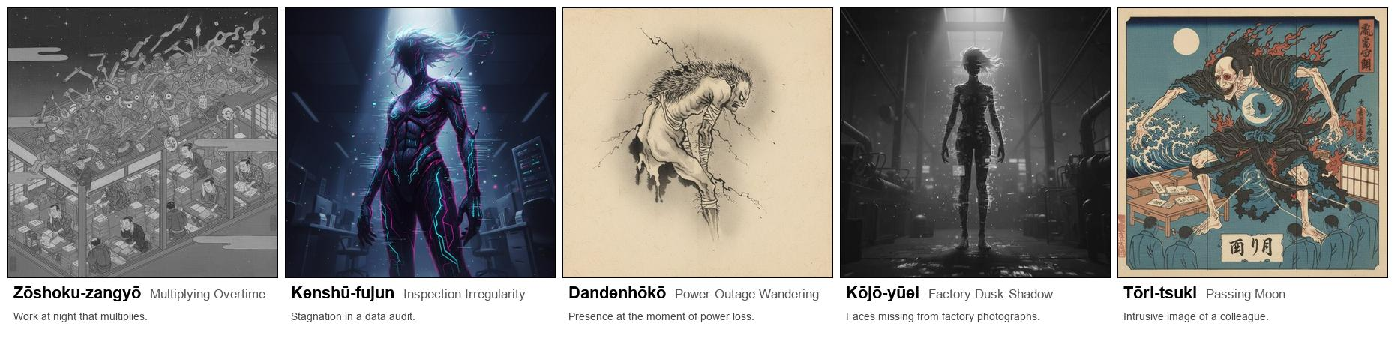
\includegraphics[width=\textwidth]{figures/fig6_contemporary_cluster.pdf}
  \caption{The five generated \textit{y\=okai} whose phenomena have no precedent in the 35{,}305-entry Nichibunken Y\=okai Database. Three (\textit{Z\=oshoku-zangy\=o}, \textit{Dandenh\=ok\=o}, \textit{T\=ori-tsuki}) sit within the apparatus's folkloric pictorial registers (woodblock and ink wash); two (\textit{Kensh\=u-fujun}, \textit{K\=oj\=o-y\=uei}) appear in the contemporary digital register, which the apparatus selects when participant accounts describe contemporary settings.}
  \label{fig:cluster}
\end{figure*}

\subsection{What Participants Reported}

The post-experience surveys document a consistent change in how participants framed \textit{y\=okai} and a less measurable but more striking change in their felt relation to the category.

Twenty-four of 36 paired pre/post responses (66.7\%) ended the encounter in a category different from where they began (Table~\ref{tab:shift}). The post-experience distribution was dominated by \textit{psychology} (18 of 36, 50\%), in which \textit{y\=okai} are understood as names given to inarticulate experience. Together with \textit{culture}, the two interpretive categories accounted for 25 of the 36 responses. All seven visitors who entered with the \textit{character} (commercial-media) framing departed from it.

\begin{table}[h]
\caption{Pre--post \textit{y\=okai} category shift (N=36). Rows: pre-experience category; columns: post-experience category. Bold diagonal: no change.}
\label{tab:shift}
\small
\begin{tabular}{p{1.6cm}cccccc|c}
\hline
\textbf{Pre} & \textbf{char.} & \textbf{cult.} & \textbf{none} & \textbf{psych.} & \textbf{scary} & \textbf{spir.} & \textbf{$\Sigma$} \\
\hline
character  & \textbf{0} & 1 & 0 & 3 & 2 & 1 & 7 \\
culture    & 1 & \textbf{5} & 2 & 8 & 1 & 1 & 18 \\
none       & 0 & 0 & \textbf{1} & 0 & 0 & 0 & 1 \\
psychology & 0 & 1 & 1 & \textbf{6} & 0 & 0 & 8 \\
scary      & 0 & 0 & 0 & 1 & \textbf{0} & 1 & 2 \\
\hline
$\Sigma$   & 1 & 7 & 4 & 18 & 3 & 3 & 36 \\
\hline
\end{tabular}
\end{table}

A forced-choice item asked which of seven thematic descriptions best matched the experience (37 respondents, up to two selections each). The two most-selected were ``making \textit{y\=okai} images with AI'' (18 of 37) and ``visualizing human fears or anxiety'' (14 of 37) — respectively the apparatus's technical means and the cultural function it was built to support.

Twenty-three substantive free-text responses converge on one description: the apparatus rendered an experience already present in the participant but not yet articulated.

\begin{quote}
\small
``Through the power of AI, I was able to give material form to phenomena I had only vaguely felt as frightening.'' (20s, general; generated \textit{K\=oj\=o-y\=uei})\\[2pt]
``A work that visualizes the anxiety and unknown emotions inside oneself when one hears the word \textit{y\=okai}.'' (40s, general; generated \textit{Tojikoshikage})\\[2pt]
``The concretization of what people today consider \textit{y\=okai}-like.'' (30s, researcher; generated \textit{Y\=ugurashioto})
\end{quote}

The participants who generated the five \textit{y\=okai} without precedent in the corpus describe exactly this transition; the cluster reported in Section~4.2 is the record of participants bringing contemporary inarticulate phenomena to the apparatus and the apparatus providing the form.

The post-survey measure of intention to investigate folklore or strange tales after the encounter (1--5 scale) gave a mean of 3.51 (SD 0.99), with 21 of 37 respondents (57\%) selecting 4 or 5.

One participant articulated a structural limitation of the apparatus directly: ``the concept of cosmic rays from outer space was rendered as image successfully, but since the \textit{aha} experience requires an \textit{aha} moment, no \textit{aha}-like image was generated.'' For experiential structures whose content is the moment of experience itself, the apparatus produced only a static depiction of a setting. Several visitors folded the printed \textit{y\=okai} and placed it in a wallet or notebook; one described the result as ``the picture given as a souvenir.''



%%% ━━━━━━━━━━━━━━━━━━━━━━━━━━━━━━━━━━━
%%% 5. REFLECTION
%%% ━━━━━━━━━━━━━━━━━━━━━━━━━━━━━━━━━━━
\section{Discussion}

\subsection{What the Contemporary Setting Cluster Suggests}

The five \textit{y\=okai} reported in Section~4.2 do not appear in the 35{,}305-entry corpus. Participants brought the underlying experiences as descriptions of their own lives, and the apparatus supplied a folkloric naming convention through which these experiences entered a vocabulary that the corpus has been collecting for centuries.

The substantive shift the cluster expresses is not contemporary content alone. Where the historical \textit{y\=okai} is encountered as an Other — a sound by a stream, a shape on a road, an animal taking unfamiliar form — the cluster's entries are characterized by the absence of a localizable supernatural agent. Work multiplies with no identifiable cause. Data stagnates without origin. A colleague's image intrudes on attention. The named entity has no distinct supernatural standing. What persists across the historical and contemporary cases is the operation of naming; what is being named has shifted from external supernatural encounter to interior felt pressure inside institutional and labor space.

The shift is structural along three dimensions. First, the loci. The cluster's entries are located in abstract zones of contemporary institutional life — the workplace at night, the audit of records, the photograph of an abandoned factory, the event venue at the moment of failure — rather than at the specific times and places (twilight, the road, the riverbank) the historical entries pair with their encounters. Second, the effects. The cluster's effects (slow drain, multiplication, stagnation) operate on the participant's attention or affect rather than on the environment, and do not require a discrete encounter event to manifest. Third, the attribution. Cause-and-effect attribution typical of historical \textit{y\=okai} (a \textit{tanuki} shape-shifts; an old woman becomes a fire) is absent: the cluster's entries record discomfort without ascribing it to a being. The historical category recorded encounter; the contemporary cluster records interior pressure under conditions of institutional life.

This is what the cluster suggests, not demonstrates: whether the entries circulate beyond their participants and whether the apparatus's mode of naming is continuous with the historical mode remain open. The narrower claim is that under apparatus-supplied conditions the naming operation attaches itself to interior contemporary unease, and the named object has structural features distinct from those that organized the historical taxonomy.

\subsection{From Communal Time to a Single Encounter}

The historical formation of a \textit{y\=okai} entry is a social process distributed across time: an experience is told, retold and varied across speakers, a variant takes hold across a region, the entry is eventually pictorialized, and a compiler records it. The sequence requires retelling, variation, communal acceptance, and historical sedimentation — none of which one person can perform.

The apparatus folds this distributed process into a single encounter of three to five minutes. The retelling, the regional sharing, and the historical sedimentation do not happen. What cultural status does the apparatus's output have, when an act historically completed across decades is completed in three to five minutes between an individual and a machine?

The output is not a transmitted \textit{y\=okai} — it carries no history of variation, no regional acceptance, no test of survival across retellings — and it is also not merely a machine-generated image. The participant brought the experience, retrieval located precedents against which it could be discussed, the models proposed a form drawn from those precedents, and the participant decided. Read in this way, the apparatus is not a machine for registering new folk entries but a device that lets an individual briefly experience the form of an act that historically belonged to communal time. What the participant takes away is not a contribution to folk tradition but the felt structure of the contribution that the tradition once consisted of.

\subsection{Limitations}

The participant population was self-selected for interest in \textit{y\=okai}; pre-survey familiarity (mean 3.26 of 5.0) confirms it is not representative of general audiences. The without-precedent claim for the five cluster entries is one of absence under this corpus and this token-level procedure, not absence in folk tradition. The apparatus depends on commercial language and image models whose behavior is subject to revision and outside the authors' control; the records here are tied to model behavior at the time of operation. The authors are not bearers of regional folk tradition, and the records and interpretations are open to revision by those who are. Finally, an apparatus that admits new named entries to a historical taxonomy risks producing material that, taken out of context, could be misread as traditional folk record; the retrieval step is intended in part as a mitigation by making explicit which historical lineage each new entry extends.


%%% ━━━━━━━━━━━━━━━━━━━━━━━━━━━━━━━━━━━
%%% 6. CONCLUSION
%%% ━━━━━━━━━━━━━━━━━━━━━━━━━━━━━━━━━━━
\section{Conclusion}

The apparatus performs the \textit{y\=okai}-naming act as a three-to-five-minute individual encounter rather than the communal accumulation across decades that the historical form required, producing 66 entries across 79 sessions of which five describe phenomena without precedent in the 35{,}305-entry corpus.

This is not a return of folk practice to its historical content. Under apparatus-supplied conditions, the naming operation attaches itself to whatever the present makes available as inexplicable, and the structural shape of what gets named departs from the encounter-on-the-road that organized the historical taxonomy. The broader research orientation the paper opens is to read a folk corpus not only as an archive of recorded entries but as a substrate against which the contemporary act of naming the inexplicable can be staged, observed, and studied as it happens.


%%% ━━━━━━━━━━━━━━━━━━━━━━━━━━━━━━━━━━━
%%% REFERENCES
%%% ━━━━━━━━━━━━━━━━━━━━━━━━━━━━━━━━━━━
\begin{thebibliography}{20}

\bibitem{bardzell2013}
Jeffrey Bardzell and Shaowen Bardzell. 2013.
What is ``Critical'' about Critical Design?
In \textit{Proceedings of the SIGCHI Conference on Human Factors in Computing Systems (CHI '13)}. ACM, New York, 3297--3306.

\bibitem{foster2009}
Michael Dylan Foster. 2009.
\textit{Pandemonium and Parade: Japanese Monsters and the Culture of Y\=okai}.
University of California Press, Berkeley.

\bibitem{foster2015}
Michael Dylan Foster. 2015.
\textit{The Book of Y\=okai: Mysterious Creatures of Japanese Folklore}.
University of California Press, Berkeley.

\bibitem{inoue1893}
Enry\=o Inoue. 1893.
\textit{Y\=okai-gaku K\=ogi} [Lectures on Y\=okai-gaku].
Tetsugakkan, Tokyo.

\bibitem{jinnai2025}
Yuto Jinnai et al. 2025.
Do Large Language Models Know Folktales? A Case Study of Y\=okai in Japanese Folktales.
\textit{arXiv preprint}. \url{https://github.com/CyberAgentAILab/YokaiEval}.

\bibitem{kagawa2020}
Masanobu Kagawa. 2020.
Kimi no Na wa: Naming \textit{Y\=okai} in the Early Modern Period.
\textit{Nihon Minzokugaku} [Journal of the Folklore Society of Japan] 302, 1--35.

\bibitem{kagawa2022}
Masanobu Kagawa. 2022.
\textit{Y\=okai o Nazukeru} [Naming the Y\=okai].
Iwanami Shoten, Tokyo.

\bibitem{sato2020}
K\=osuke Sato and Y\=o Nakawake. 2020.
Minkan Densh\=o no Keiry\=o Bunseki: \textit{Kaii-Y\=okai Densh\=o D\=etab\=esu} no Fukan-teki Bunseki [Quantitative Analysis of Folk Tradition: A Statistical Overview of the \textit{Kaii-Y\=okai} Tradition Database].
In \textit{Jinmonkon 2020 Proceedings} [Symposium on Humanities and Computer, IPSJ], 30--37.

\bibitem{iikura2025}
Yoshiyuki Iikura. 2025.
\textit{Gendai o Ikiru Kaii Y\=okai} [\textit{Kaii} and \textit{Y\=okai} Living in the Present].
In \textit{Kaii Y\=okai-gaku Korekushon} [Collection of \textit{Kaii Y\=okai} Studies], Vol.~3, Kazuhiko Komatsu (Ed.). Seikyusha, Tokyo.

\bibitem{hirota2017}
Ry\=uhei Hirota. 2017.
Y\=okai Studies in the Age without \textit{Kami}.
\textit{Journal of Living Folklore} 9, 43--62.

\bibitem{ichikawa2014}
Hiroya Ichikawa. 2014.
\textit{Y\=okai Bunka no Gendai-teki Katsuy\=o ni kansuru Kenky\=u: Chiiki J\=umin o Shutai to suru Y\=okai Sonzai no Sais\=oz\=o no Jirei kara} [On Contemporary Uses of Y\=okai Culture: Cases of Y\=okai Re-Creation Led by Local Residents].
Doctoral dissertation, University of Tsukuba.

\bibitem{komatsu2011}
Kazuhiko Komatsu. 2011.
Y\=okai to wa nani ka [What are Y\=okai?]. In \textit{Y\=okai-gaku no Kiso Chishiki} [Foundations of Y\=okai-gaku], Kazuhiko Komatsu (Ed.). Kadokawa Gakugei Shuppan, Tokyo, 9--31.

\bibitem{miyata1985}
Noboru Miyata. 1985.
\textit{Y\=okai no Minzokugaku: Nihon no Mienai K\=ukan} [Folklore of Y\=okai: The Invisible Space of Japan].
Iwanami Shoten, Tokyo.

\bibitem{tsunemitsu1993}
T\=oru Tsunemitsu. 1993.
\textit{Gakk\=o no Kaidan: K\=osh\=o Bungei no Tenkai to Sh\=os\=o} [School Ghost Stories: Development and Aspects of Oral Folklore].
Minerva Shob\=o, Kyoto.

\bibitem{komatsu2017}
Kazuhiko Komatsu. 2017.
\textit{An Introduction to Y\=okai Culture: Monsters, Ghosts, and Outsiders in Japanese History}.
Japan Publishing Industry Foundation for Culture (JPIC), Tokyo.
Trans. Hiroko Yoda and Matt Alt.

\bibitem{mirowski2023}
Piotr Mirowski, Kory W. Mathewson, Jaylen Pittman, and Richard Evans. 2023.
Co-Writing Screenplays and Theatre Scripts with Language Models: Evaluation by Industry Professionals.
In \textit{Proceedings of the 2023 CHI Conference on Human Factors in Computing Systems (CHI '23)}. ACM, New York.

\bibitem{nichibunken_db}
International Research Center for Japanese Studies (Nichibunken).
Y\=okai Database (publicly accessible).
\url{https://www.nichibun.ac.jp/youkaidb/}. Accessed 2026.

\bibitem{ozawa2024}
Chinatsu Ozawa, Tatsuya Minagawa, and Yoichi Ochiai. 2024.
Can AI Generated Ambrotype Chain the Aura of Alternative Process?
In \textit{SIGGRAPH Asia 2024 Art Papers}. ACM, New York.

\bibitem{sekien1776}
Toriyama Sekien. 1776.
\textit{Gazu Hyakki Yagy\=o} [The Illustrated Night Parade of a Hundred Demons].
Woodblock-printed volumes. Edo (Tokyo).

\bibitem{sfpc_decay}
The School for Poetic Computation (SFPC).
The Emergence and Decay of Computation.
Installation documentation. \url{https://sfpc.study}. Accessed 2026.

\bibitem{tanaka1994}
Takako Tanaka. 1994.
\textit{Hyakki Yagy\=o no Mieru Toshi} [The City Where Hyakki Yagy\=o Is Visible].
Shin'y\=osha, Tokyo.

\bibitem{tsuji1970}
Nobuo Tsuji. 1970.
\textit{Kis\=o no Keifu} [Lineage of Eccentrics].
Bijutsu Shuppansha, Tokyo. Reissued 2004, Chikuma Shob\=o.

\bibitem{walton1970}
Kendall L. Walton. 1970.
Categories of Art.
\textit{The Philosophical Review} 79, 3, 334--367.

\bibitem{yanagita1956}
Kunio Yanagita. 1956.
\textit{Y\=okai Dangi} [Discussions on Y\=okai].
Shueisha, Tokyo.

\bibitem{yokai_com}
Matthew Meyer. n.d.
yokai.com: An online database of Japanese ghosts and monsters.
\url{https://yokai.com}. Accessed 2026.

\end{thebibliography}


\section*{AI Tools Disclosure}
Large Language Models were used to assist in the research planning and linguistic editing of this manuscript. The generative AI components described in the system (retrieval-augmented generation, image synthesis) are part of the artwork itself. All conceptual design, system implementation, exhibition deployment, observational analysis, and interpretive conclusions were conducted by the human authors, who assume full responsibility for the content.

\end{document}
